\documentclass{article}
\usepackage{enumitem}
\usepackage{geometry}
\usepackage{array}
\usepackage{pdfpages}
\usepackage{float}
\usepackage{tabularx}
\usepackage[export]{adjustbox}
 \geometry{
 a4paper,
 left=20mm,
 right=20mm,
 top=25mm,
 bottom=20mm
 }
 
\newlist{legal}{enumerate}{10}
\setlist[legal]{label*=\arabic*.}

\begin{document}
	
	\begin{figure}
  	
\includegraphics[width=\linewidth]{../images/Logo-PoliMi.jpg}
	\end{figure}
	\title{\textbf{Software Engineering 2\\Design Document}}
	\author{Work team:\\Paolo Romeo, Andrea Scotti, Francesco Staccone}
	\date{AY 2018-2019}
	\maketitle{}

	\newpage
	
	\textbf{Table of contents}

	\begin{legal}
 	\item Introduction
  		\begin{legal}
    		\item Purpose
		\item Scope
		\item Definitions, acronyms, abbreviations
		\item Revision history
		\item Reference documents
		\item Document structure	
  		\end{legal}
	\item Architectural design
  		\begin{legal}
    		\item Overview:High-level components and their interaction
		\item Component view
		\item Deployment view
		\item Runtime view
			\begin{legal}
			\item Sign up Runtime View
			\item Login Runtime View
			\item Join a run Runtime View
			\item Organise a run Runtime View
			\item Individual request Runtime View
			\item Group request Runtime View
	  		\end{legal}
		\item Component interfaces
			\begin{legal}
			\item REST API
	  		\end{legal}
		\item Selected architectural styles and patterns
  		\end{legal}
	\item User interface design
  		\begin{legal}
    		\item UX Diagram
  		\end{legal}
	\item Requirements traceability
	\item Implementation, integration and test plan
  	\item Effort spent
	\item References
	\end{legal}
	
	\newpage
	\begin{legal}
	\item {\pagenumbering{gobble}
	\underline{\textbf{Introduction} }
	\begin{legal}
    		\item \textit{\textbf{Purpose}}\\\\
		This document is thought to be an overview of the TrackMe application, in which is explained how to satisfy the several project requirements stated in the RASD. This document is principally intended for the developers and the testers, with the purpose of providing a functional description of the main architectural components, their interfaces and their interactions, along with the design patterns.\\
		\item \textit{\textbf{Scope}}\\\\
		The TrackMe system is thought to be a Health Data Management and Run-Friendly Mobile App, useful for a quite wide range of users with different features and necessities. The software will be made up of three different modules: Data4Help, a service that allows the third parties to monitor the location and the health status
of the individuals; AutomatedSOS , an optional service that monitors the health status of the users by performing
a continuous evaluation of the health parameters' data acquired by Data4Help; Track4Run, a service thought for the organization of running events.\\ 
		To provide the previous services in the best way, the overall system is structured in a multi-tier architecture. More specifically, the Business logic layer has the task of taking charge of the incoming requests/data, computing checks, and interacting with external third-party services through the use of interfaces. This layer is connected with the Data layer, in which are stored all the Users data (credentials, health data). The Presentation layer is build through the hybrid Client paradigm in which the client needs to perform computation for the partial analysis and filtering of incoming data. \\
		\item \textit{\textbf{Definitions, acronyms, abbreviations}}\\
			\begin{legal}
				\item \textbf{Definitions}\\
				\begin{itemize}
					\item User: a registered individual who can use the TrackMe services.
					\item Third party: a registered entity that can use the TrackMe services.
					\item Client: A client is a piece of computer hardware or software that accesses a service made available by a server;
					\item Firewall: A network security system that monitors and controls incoming and outgoing network traffic based on predetermined security rules;
					\item Server: A computer program or a device that provides functionality for other programs or devices, called "clients".\\
				\end{itemize}
				\item \textbf{Acronyms}\\
				\begin{itemize}
					\item API: Application Program Interface;
					\item DBMS: Database Management System;
					\item DD: Design Document
					\item GUI: Graphical User Interface;
					\item HTTP: Hypet Text Transfer Protocol;
					\item MVC: Model View Controller pattern;
					\item OS: Operating System;
					\item RASD: Requirements Analysis and Specifications Document;
					\item REST: REpresentational State Transfer;\\
				\end{itemize}
				\item \textbf{Abbreviations}\\
				\begin{itemize}
					\item Gn: n-goal in the RASD;
					\item Rn: n-functional requirement in the RASD;\\\\\\
				\end{itemize}
			\end{legal}
		\item \textit{\textbf{Revision history}}\\
			\begin{itemize}
				\item 10/12/2018		Version 1.0\\
			\end{itemize}
		\item \textit{\textbf{Reference documents}}\\
			\begin{itemize}
				\item RASD document;
				\item Mandatory project assignment;
				\item Slides of the lessons.\\
			\end{itemize}
		\item \textit{\textbf{Document structure}}\\\\
		The following document is organised in this way:
		\begin{itemize}
				\item Architectural Design: this section shows the main components of the system and the connections among them. It will also focus on design choices, styles and patterns.
				\item User Interface Design: this section includes an improvement of the user interface given in the RASD document. It will be described through the use of UX modeling.
				\item Requirements Traceability: this section shows how the requirements in the RASD are mapped to the design components presented in the DD;
				\item Implementation, Integration and Test plan: this section shows the order in which the implementation and the integration of the subcomponents will occur and how the integration will be tested.\\\\
			\end{itemize}
  	\end{legal}

}
	\newpage
	\item{\pagenumbering{gobble}
	\underline{\textbf{Architectural design} }
	\begin{legal}
    	\item \textit{\textbf{Overview: high-level components and their interaction}}\\\\
The figure below represents an high level overview of the system. Further details
on the system components and their interaction will be further explained in the next sections.\\
		\begin{figure}[H]
		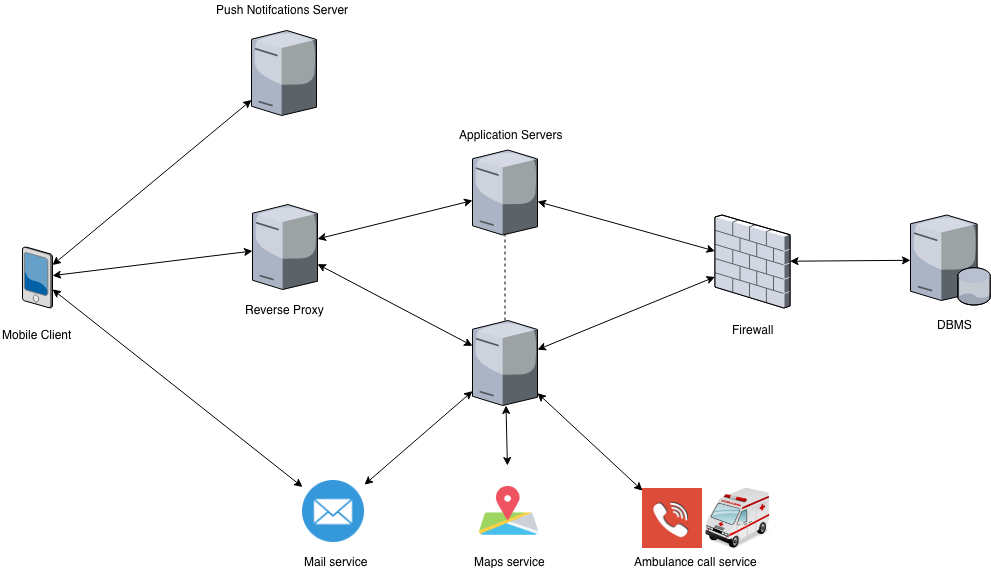
\includegraphics[width=\linewidth]{../images/design/OverviewDiagram.png}
		\end{figure}
		
		\item \textit{\textbf{Component view}}\\\\
		\begin{figure}[H]
		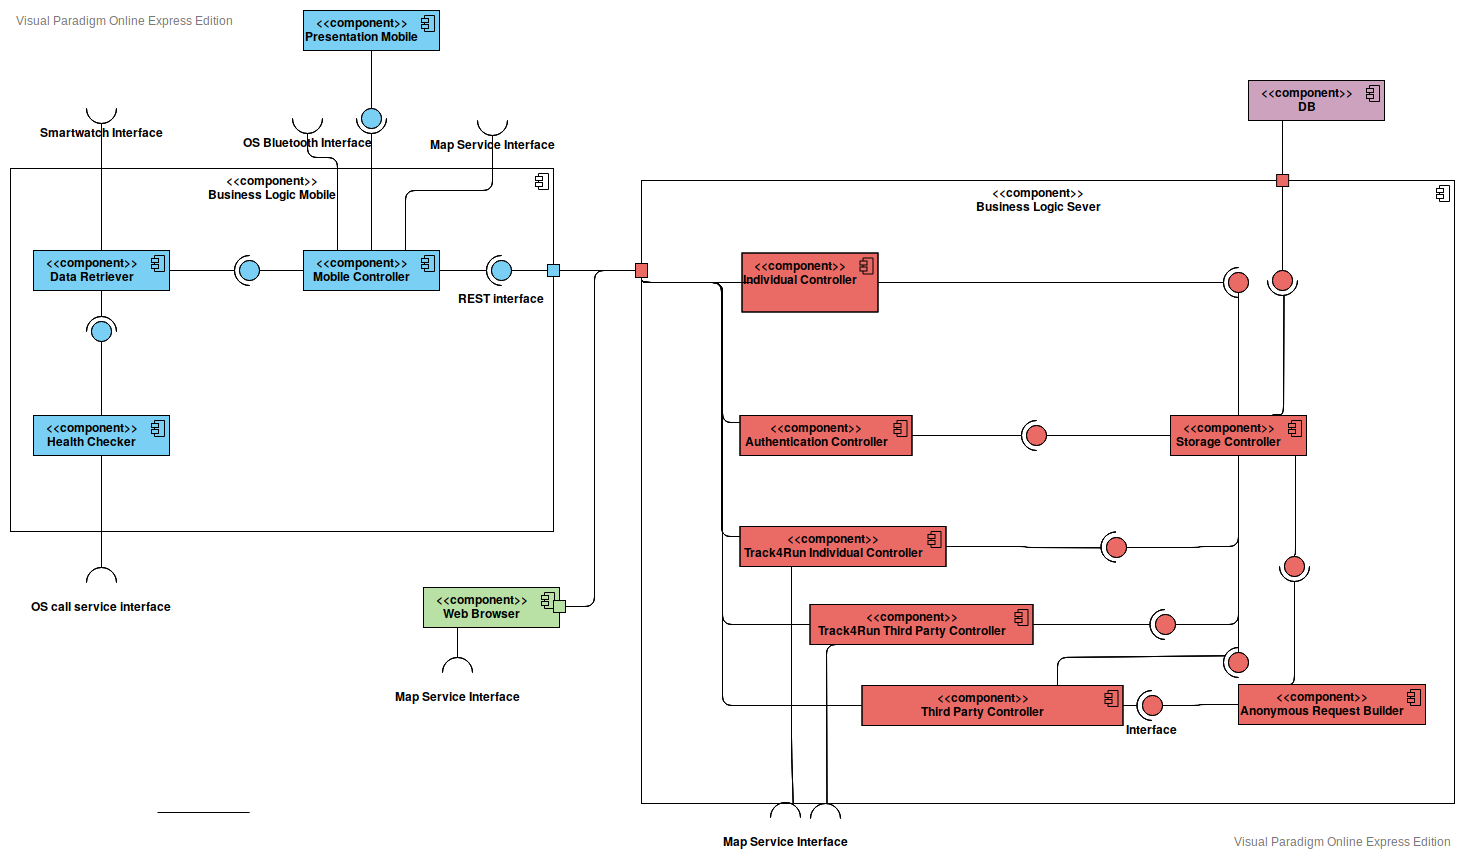
\includegraphics[width=\linewidth]{../images/design/ComponentDiagram.png}
		\end{figure}
		The UML component diagram shows the internal structure of the system highlighting the individual modules and the connections among them. Individual components are wired together by using an assembly connector to connect the required interface of one component with the provided interface of another component. Below is the description of the components:\\
		\begin{itemize}
		\item{\textbf{User mobile client}\\
		This is the component that represents the client machine that accesses to the API of the Business Logic container for the user. ???????????????????????? Da completare in base a come lo vogliamo implementare (dati lato utente o no?)
				}\\
		\item{\textbf{Third party mobile client}\\
		This component represents the client machine that accesses to the API of the Business Logic container for the third party. ????????????????????????????????
				}\\
		\item{\textbf{User controller}\\
		The main role of this component is to manage the transfer of data from the client to the server using the interface provided by the Data component. It also provides methods to accept/refuse a request of agreement and to change login credentials. It can communicate with the Notification controller component to display notifications.
				}\\
		\item{\textbf{Third party controller}\\
		This component is built to manage the transfer of data from the system to the third party using the interface provided by the Data component. It also provides methods to send requests of agreement and requests of data to the system. It can communicate with the Notification controller component to display notifications.
				}\\
		\item{\textbf{Authorization controller}\\
		This component provides authentication and registration processes for both the users and the third parties. It takes the needed data from the Data component and communicates the result of the operations trough the Notification controller.
				}\\
		\item{\textbf{User run controller}\\
		This component provides the methods to permit a user to join, leave, check and watch a run. It communicates with the external service that provides maps trough the Map services interface. Every time a user wants to join a run, it calls the Feasability checker that checks if all the constraints are satisfied. Finally, it can access data of the runs trough the Data component and it can call the Notification controller to send notifications.
				}\\
		\item{\textbf{Third party run controller}\\
		This component provides the methods to allow a third party to organize a run. It communicates with the external service that provides maps trough the Map services interface to allow the third party to select the track for the run.
				}\\				
		\item{\textbf{Notification controller}\\
		This component manages the notifications forwarded by the other components. It only shows notifications inside the application.
				}\\
		\item{\textbf{Health checker}\\
		This component is the core of the service AutomatedSOS. It receives data from the Data component, elaborates them and, if needed, communicates to the Call service interface to send an SOS trough the related external service.
				}\\
		\item{\textbf{Feasability checker}\\
		This component is built to check if a user can actually join a run that is shown trough the Mobile client.
		----------- Serve davvero??????????????????????????????????
				}\\
		\item{\textbf{Data}\\
		The Data component provides the set of Classes corresponding to the tables contained in the Database.
				}\\
		\item{\textbf{Storage interface}
		This component provides the methods for querying the Database.
				}\\
		\item{\textbf{Database}
		This component represent the DBMS. It provides the interfaces to retrieve and store data. In the database there are data about users, third parties and the set of agreements among them. It also contains data about the runs.
				}\\
		\item{\textbf{External services interfaces}\\
      	\begin{itemize}
      	\item{\textbf{Map services interface}\\\
      	It communicates with the map service to allow the third party to select the track and to show the position of runners in real time on the map.
					}\\
			\item{\textbf{Call service interface}\\
			It communicates with the external service to dispatch automatic calls (or emails?) in case of emergency.
					}\\
      	\end{itemize}
				}
		\end{itemize}

		\item \textit{\textbf{Deployment view}}\\\\
		The figure below shows the deployment diagram of the whole system. Its main goal is to describe the distribution of components capturing the topology of the
system's hardware.\\
		\begin{figure}[H]
		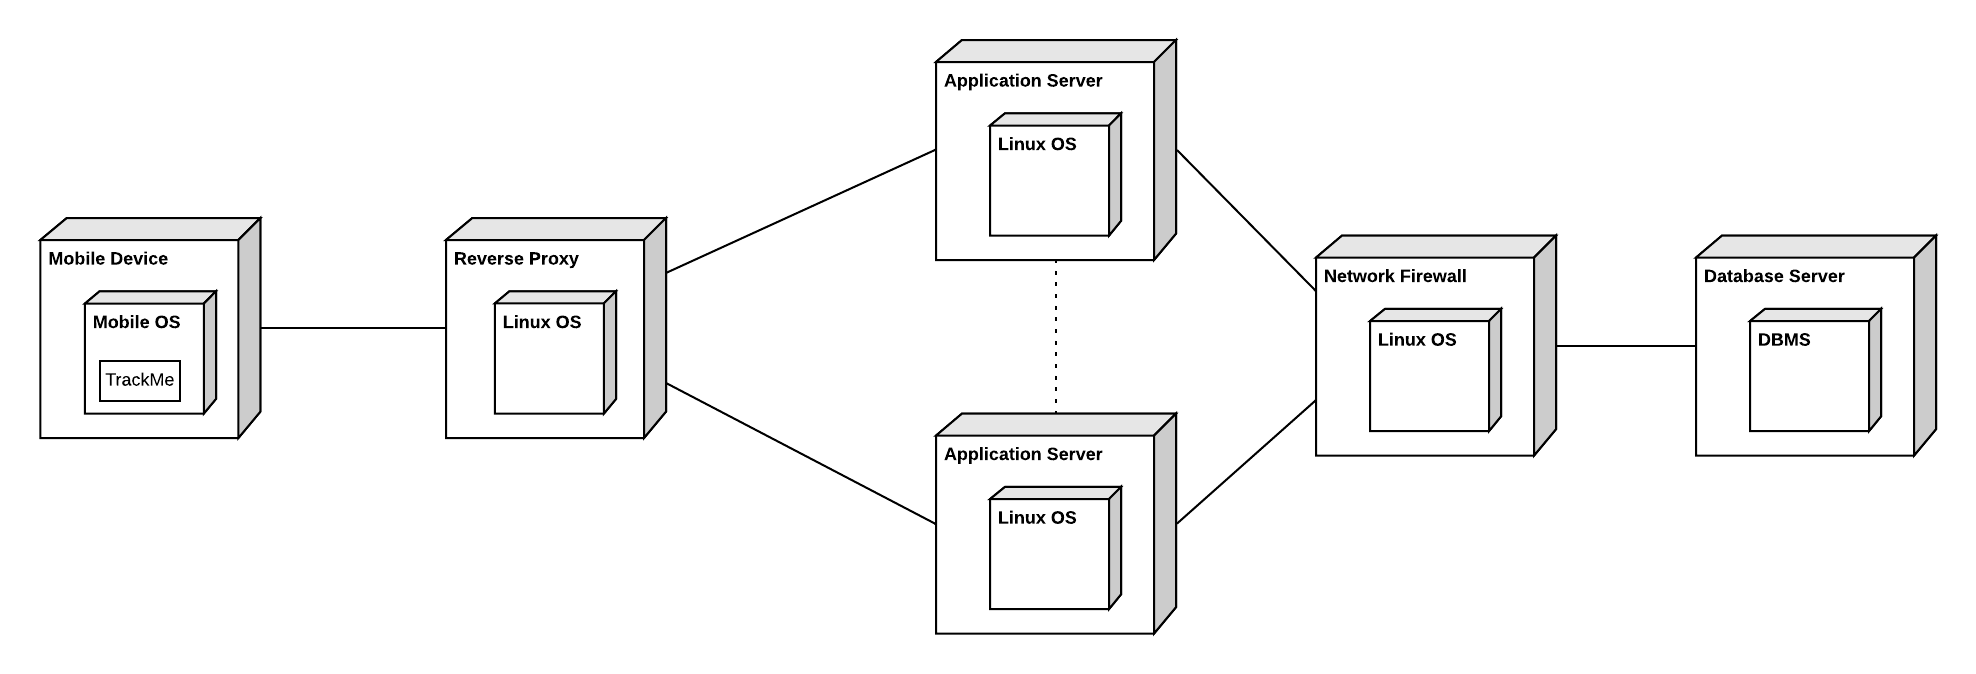
\includegraphics[width=\linewidth]{../images/design/DeploymentDiagram.png}\\
		\end{figure}
		As previously stated in the section 1, the system is structured in a multi-tier architecture. The specific role of each node is clarified here:\\\\
		\textbf{Clients}\\
The first tier is composed by the clients machines (mobile for individuals and desktop for third parties). The individuals will be able to access TrackMe functionalities through the dedicated native application while the third parties through any web browser.\\\\
		\textbf{Application Server}\\
This is the middleware level of the architecture: all the business logic of
the system is contained in this server.\\\\
		\textbf{Network Firewall}\\
The access to the Database is mediated by a network firewall in order to
avoid unauthorised access to the data and the credentials of the user.\\\\
		\textbf{Database Server}\\
This is the last layer of the architecture: all the data are stored in a Database Server accessed through a relational DBMS. \\\\

		\item \textit{\textbf{Runtime view}}\\
			\begin{legal}
				\item \textbf{Sign up Runtime View}\\
				\item \textbf{Login Runtime View}\\
				\item \textbf{Join a run Runtime View}\\
				\item \textbf{Organise a run Runtime View}\\
				\item \textbf{Individual request Runtime View}\\
				\item \textbf{Group request Runtime View}\\
			\end {legal}
		\item \textit{\textbf{Component interfaces}}\\\\
		\item \textit{\textbf{Selected architectural styles and patterns}}\\\\
  	\end{legal}
}
	\newpage
	\item{\documentclass{report}
\usepackage{enumitem}
\usepackage{geometry}

\newlist{legal}{enumerate}{10}
\setlist[legal]{label*=\arabic*.}

 \geometry{
 a4paper,
 left=20mm,
 right=20mm,
 top=25mm,
 bottom=20mm
 }

\pagenumbering{gobble}

\begin{document}
	\underline{\textbf{User interface design}}
\end{document}}
	\newpage
	\item{\pagenumbering{gobble}
	\underline{\textbf{Requirements traceability}}\\\\
	\begin{itemize}
		\item \textbf{Third Party Controller}
		\begin{itemize}
			\item R2) The system must be able to provide to the third party the location and the health status of individuals;
			\item R9) The third party is not allowed to access the user’s data until he/she accepts the request.\\
			\item R11) The system is optimized to send the data received from the mobile application to the third parties as soon as possible.\\
		\end{itemize}
		\item \textbf{Anonymous Request Builder}
		\begin{itemize}
			\item R4) The groups must be composed at least by 1000 individuals;\\
			\item R5) The system must be able to provide to the third party the health status of individuals in an anonymous way;\\
			\item R6) The system must be able to aggregate the data of the individuals, as requested by the third party;\\
		\end{itemize}
		\item \textbf{Data Retriever}
		\begin{itemize}
			\item R3) The system must be able to retrieve data from the smartwatches and similar devices;\\
		\end{itemize}
		\item \textbf{Storage Controller}
		\begin{itemize}
			\item R27) The system must be able to store data retrieved from registered users.\\
			\item R8) The system must save the preference of the user;\\
		\end{itemize}
		\item \textbf{Individual Controller}
		\begin{itemize}
			\item R1) The users must have given the consensus to the treatment of their information to the third party;\\
			\item R28) The user must have an active subscription to stop it;\\
	 		\item R29) The system must be able to allow the user to unsubscribe to the third party and to stop the transmission of his/her data.\\
	 		\item R7) The system must be able to forward the requests from the third party to the user;\\
	 		\item R26) The system must allow the user to enable/disable the AutomatedSOS service at any time.\\
			\item R31) The system must allow the user to change his/her personal info.\\
		\end{itemize}
		\item \textbf{Authentification Controller}
		\begin{itemize}
			\item R12) The individual must provide their personal data to the application during the registration process, SSN (or fiscal code) included;\\
			\item R13) The system must allow the individual to register to the application by selecting a username and a password;\\
			\item R14) The system must allow the individual to log in to the application by providing the combination of a username and a password that matches an account;\\
			\item R15) Two different users cannot have the same username.\\
			\item R16) The system must allow the third party to register to the application, by specifying its VAT registration number and a password;\\
			\item R17) The system must allow the third party to log in to the application by providing the combination of a VAT registration number and a password that match an account;\\
			\item R32) The system must allow the individual to change his/her password.\\
			\item R33) The system must allow the Third party to change its password.\\
		\end{itemize}
		\item \textbf{Track4Run User Controller}
		\begin{itemize}
			\item R19) The system must be able to retrieve the position of all the runners;\\
			\item R20) The system must be able to provide the position of all the runners in the track in real time.\\
			\item R21) The system must allow the user to check the list of available races at any time.\\
			\item R22) The system must allow the user to join an available race only before its starting time.\\
			\item R23) The user cannot join two different overlapping races.\\
			\item R30) The system must avoid the registration of users after having reached of the maximum number of participants.\\
		\end{itemize}
		\item \textbf{Track4Run Third Party controller}
		\begin{itemize}
			\item R19) The system must be able to retrieve the position of all the runners;\\
			\item R24) The system must allow the third party to organize a race by defining its track and its time.\\
		\end{itemize}
		\item \textbf{Health Checker}
		\begin{itemize}
			\item R18) When the health status values go below the threshold, the system must send an SOS within 5 seconds.\\
			\item R25) The AutomatedSOS service must be enabled.\\
		\end{itemize}
		\item \textbf{Mobile Controller}
		\begin{itemize}
			\item R34) The system must allow the user to connect a smartwatch or a similar device to its smartphone.\\
		\end{itemize}
	\end{itemize}
	
}
	\newpage
	\item{\pagenumbering{gobble}
	\underline{\textbf{Implementation, integration and test plan}}\\\\
In section 2.2 of this document there is the description of the components in which the whole system can be divided to split roles and functionalities and to simplify the development and the following testing.
As it is evident from the Component Diagram, the components can be classified into the following subsystems:
	\begin{itemize}
	\item Mobile client, made up by:
		\begin{itemize}
		\item Components: Mobile controller,  Data retriever, Health checker, Presentation mobile;
		\item Interfaces for external services: Map service interface, OS Bluetooth interface, Smartwatch interface, OS call service interface.
		\end{itemize}
	\item Web client: browser and Map service interface.
	\item Business logic, made up by:
		\begin{itemize}
		\item Components: Individual controller, Third party controller, Authentication controller, Track4Run Individual controller, Track4Run Third party controller, Anonymous request builder, Storage controller;
		\item Interfaces for external services: Map service interface.
		\end{itemize}
	\item External components: Map service, OS Bluetooth service, OS call service, Smartwatch service, DBMS.\\
	\end{itemize}

A bottom-up strategy will be used to implement, integrate and test the system.
Firstly single components have to be implemented and then unit tested. Later the following steps will be performed:
	\begin{enumerate} 
	\item each subsystem will be implemented, integrated and tested;
	\item the subsystems will be integrated and tested togheter.\\
	\end{enumerate}
Since we cannot directly manage external components, we assume they are reliable and we use the provided interfaces to test our system.\\

To keep the integration and testing process more clear we can split the Business logic subsystem into the following subsystems, based on their main functionalities:
	\begin{itemize}
	\item Individual subsystem: Individual controller and Storage controller;
	\item Authentication subsystem: Authentication controller and Storage controller;
	\item Thin third party subsystem: Third party controller and Storage controller;
	\item Full third party subsystem: Third party conroller, Anonymous request builder and Storage controller;
	\item Track4Run individual subsystem: Track4Run individual controller and Storage controller;
	\item Track4Run third party subsystem: Track4Run third party controller and Storage controller.\\
	\end{itemize}

To reach the same goal, in the Mobile client subsystem we can distinguish:
	\begin{itemize}
	\item AutomatedSOS subsystem: Data retriever and Health checker;
	\item Transfer data subsystem: Data retriever and Mobile controller.\\
	\end{itemize}

Focusing the attention on the Mobile client, after having tested all the subsystems (step 1), it is needed to test the integration of all of them. Let's call the result Mobile client subsystem.
	\begin{figure}[H]
	\centering
	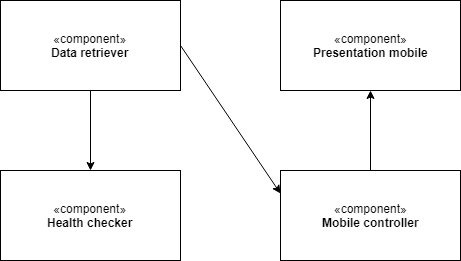
\includegraphics[scale=0.5] {images/integration/mobileClient.png}
	\caption {Mobile client subsystem}
	\end{figure}
	
Coming to the server side, after having implemented and tested all the subsystems, it is needed to test the integration of each of them with the Mobile client subsystem and with the Web client component.
More in detail:
	\begin{itemize}
	\item Mobile client subsystem and Individual subsystem;
	\item Mobile client subsystem and Authentication subsystem;
	\item Mobile client subsystem and Track4Run individual subsystem;
	\item Web client component and Authentication subsystem;
	\item Web client component and Full third party subsystem;
	\item Web client component and Track4Run third party subsystem.
	\end{itemize}
	
	\begin{figure}[H]
	\centering
	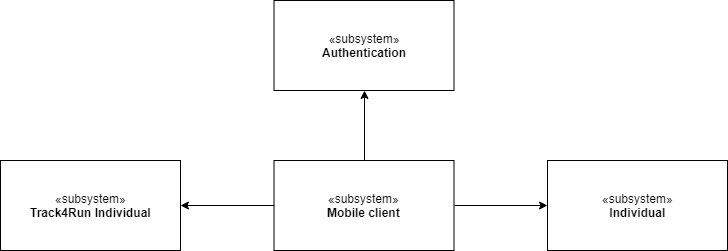
\includegraphics[scale=0.5] {images/integration/mobileAndServices.png}
	\caption {Mobile client tested with the other subsystems}
	\end{figure}
	
	\begin{figure}[H]
	\centering
	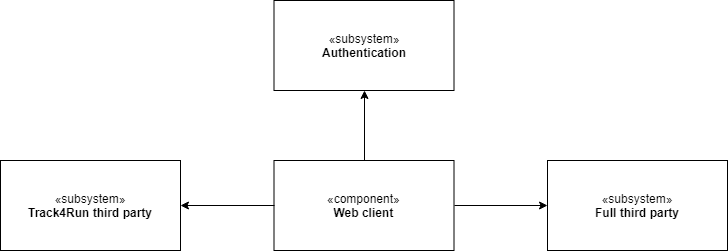
\includegraphics[scale=0.5] {images/integration/webAndServices.png}
	\caption {Web client tested with the other subsystems}
	\end{figure}
	
	After all the previous tests, a full integration test can be performed.
	
	\begin{figure}[H]
	\centering
	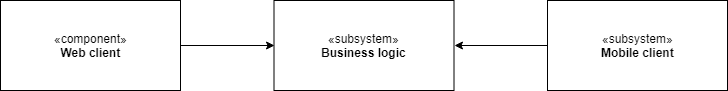
\includegraphics[scale=0.5] {images/integration/general.png}
	\caption {Test of the whole system}
	\end{figure}
	}
	\newpage
	\item{\pagenumbering{gobble}
	\underline{\textbf{Effort spent}}
}
	\newpage
	\item{\pagenumbering{gobble}
	\underline{\textbf{References}}}
	\end{legal}
\end{document}
